
\section{Material and methods}

\subsection{Simulation setup}

The monitoring system consists of a beam hodoscope and Compton prototypes under development within a French collaboration (CLaRyS - Contr\^ole en Ligne avec Rayonnements Secondaires) including five institutions: IPN Lyon, CREATIS Lyon, LPC Clermont-Ferrand, CPP Marseille and LPSC Grenoble. The detectors characteristics can be found in \cite{krimmer_development_2015}. For the sake of simplicity, the beam hodoscope is not modeled in this study to focus on PG detection. A scheme of the simulation setup is given in Figure~\ref{fig:fig_setup_CC_simulation_Hadronth}.

\begin{figure} [!hbtp]	
  \centering
  \includegraphics[width=0.7\textwidth]{./Figure/Compton_Camera_hadontherapy_PMMA_Cylinder_EN.pdf}
	  \caption{Modelling of the patient (PMMA cylinder) and the Compton camera prototype. This configuration is used for all the results presented in this paper.}
  \label{fig:fig_setup_CC_simulation_Hadronth}
\end{figure}

Like most Compton camera devices, the CLaRyS prototype uses a scatterer and an absorber. The scatterer consists of seven parallel planes of silicon detectors (double-sided silicon strip detectors, DSSD) , $9\times9\times0.2$~cm$^3$, with 1~cm distance between the centers of two neighboring planes while the absorber is a array of $10\times10$ BGO blocks ($3.5\times3.5\times3.0$~cm$^3$ each block) placed at 40~cm from the last silicon layer. A cylindrical PMMA\footnotemark[1] phantom is placed in front of the Compton camera to mimic the patient body. This cylinder of 15~cm in diameter and 20~cm in length is set at 20 centimeters in order to fit with a realistic distance to the patient.

Regarding spatial resolution\dots\com{Detail here how the spatial resolution is modeled (see Mattia's paper.}

\footnotetext[1]{PolyMethylMethAcrylate}
\footnotetext[2]{Bismuth Germanate} 

\subsection{Hadronic models used in Geant4}

The study is based on the Monte Carlo methods with the Geant4 toolkit, version 9.6 patch 02. Geant4 has been developed by the CERN for the high energy physics experiments. It was shown that it could also be used in ion therapy studies \cite{cirrone_hadrontherapy_2011,toshito_new_2010}. However, some improvements remains to do in order to adjust the hadronic models \cite{dedes_assessment_2014} .
The interaction processes in the matter are described by means of different models according to the type of particles. A resume of those different models is given table \ref{table:table_modele_physic_CC_simulation_Hadronth}. Additionally, the Doppler broadening and the polarization is taking into account. 

\definecolor{Gray}{gray}{0.9}

\begin{table}[ht]
\label{physlist_ion}
\caption{Hadronic models used in the simulations Geant4.}
\begin{scriptsize}
\begin{center}
\renewcommand{\arraystretch}{1.2}
%\begin{tabular} {>{\columncolor[gray]{0.9}}cccc}\hline  
\begin{tabular} {cccc}\hline
%\rowcolor{Gray}
\textbf{Processus} & \textbf{Protons} & \textbf{Ions} & \textbf{Neutrons} \\ \hline 
\textbf{Electromagnetic} & \multicolumn{3}{c}{standard$_{\rm{option3}}$} \\ %\hline
\textbf{Inelastic} & G4BinaryCascade & G4QMDReaction  &  G4BinaryCascade  \\ 
 & & (G4IonsShenCrossSection)&+ G4NeutronHPInelastic ($<$19 MeV)\\ %\hline
\textbf{Elastic} & G4LElastic & G4LElastic & G4LElastic + G4NeutronHPElastic ($<$19 MeV)\\ %\hline
\textbf{Fission} & / & / & G4LFission + G4NeutronHPFission($<$19 MeV) \\ %\hline
\textbf{Capture} & / & / & G4LCapture +  G4NeutronHPCapture ($<$19 MeV) \\ %\hline
\textbf{Radioactivedecay} & / & G4Radioactivedecay & / \\ \hline
\end{tabular}
\end{center}
\end{scriptsize}
\label{table:table_modele_physic_CC_simulation_Hadronth}
\end{table}

\subsection{Particles of interest}
\label{subsection:Particules_Etudiees_CC_hadrontherapy_Geant4}

We study the two main particles used in clinics, namely the protons and the carbon ions. The ion range of interest is 15.2 cm in the PMMA target. The energy associated with the range is 160 MeV for the protons and 305 MeV/n for the carbon ions. The beam delivered during a real treatment has a Gaussian profile at the enter of the patient. The standard deviation for a proton beam is 5 mm at 160 MeV and 3.5 mm for a carbon ion beam at 305 MeV/n. The modelling of the Compton camera does not change with the type of incident particles. The statistic for a spot in pencil beam scanning (PBS) mode for protons is $10^8$ particles and $10^5$ particles for carbon ions. The beam time structure is applied during the post treatment.\newline


\subsection{Data treatment}
\label{subsection:Treatment_data_CC_hadrontherapy_Geant4}

\subsubsection{Detector resolutions}
\label{subsubsection:Resolution_detector_CC_hadrontherapy_Geant4}

The Monte Carlo simulation parameters are as close to reality as possible in order to get relevant results. The detector resolutions play an important role in the Compton camera performances. The absorber's spatial resolution influences the position of the apex of the Compton cone and influences its axis orientation. The energy resolution has effect on the  Compton cone aperture angle and the timing resolution impacts the coincidence windows between the absorber and the scatterer. The hodoscope is not included in the simulation but its timing resolution is taking into account for the time of flight discrimination. The detector resolutions are modelled in relation to the resolutions measured or estimated for each detector. The spatial resolution, the energy resolution and the timing resolution are presented in the table \ref{table:table_resolution_detecteurs_CC_simulation_Hadronth}.

\begin{table} [!htbp]
\centering
%\begin{tabular}{>{\columncolor[gray]{0.9}}ccc}
\caption{Realistic resolutions applied during the simulations.}
\begin{tabular}{cccc}
\hline
\textbf{Resolution (FWHM) at 1 MeV} & \textbf{Scatterer} & \textbf{Absorber} &\textbf{Hodoscope}\\
\hline 
\textbf{spatial [mm]	}			 &     0.9		 &  5	 			&   /	\\
%\hline
\textbf{energy [\%]}				&	2.3		&  17				&   /     \\
%\hline
\textbf{timing [ns]}	        			&	15		&	3 			&  1     \\
\hline
\end{tabular}
\label{table:table_resolution_detecteurs_CC_simulation_Hadronth}
\end{table}

\subsubsection{Modelling of the ion beam structure}
\label{subsubsection:modelisation_fasceau_ions_CC_hadrontherapy_Geant4}
 


The beam time structure should have a direct impact on the Compton camera capacities to detect a particle in coincidence between the scatterer and the absorber.
Two beam time structures have been modelled: one of IBA cyclotron C230 for protons (used in 16 clinical centers worldwide) and one of synchrotron installed at the Heidelberg Ion Therapy Center (HIT) in Germany for carbon ions. Depending on the ion energy and the beam intensity, the beam microstructure will change. We are focusing in this study to the microstructure at a specific energy and also at the influence of the variation of the intensity. In the case of protons at 160 MeV, the ions are grouped in bunches of 2 ns at a frequency of 106 MHz (9.42 ns) \cite{f_roellinghoff_real-time_2014}. The clinical beam intensity is 3.2 nA which corresponds to about 200 protons per bunch. Concerning the carbon ion beam at 305 MeV/u, the estimated microstructure is a bunch of 30 ns at a frequency of 5.9 MHz (170 ns). The clinical beam intensity for carbon ions is $5\times10^7$ ions/s which corresponds to about 9 ions per bunch. This beam structure is extrapolated from measurements done by our team in 2013 at HIT. The time beam structure was measured for 200 MeV/u and 400 MeV/u carbon ion beams with a two scintillating fiber hodoscope and the spill signal given by the accelerator. The figure \ref{fig:fig_structure_temps_faisceau_HIT_2013_CC_simulation_Hadronth} shows the beam structure for carbon ions at 400 MeV/u. The pulses have a spill period of 150.2 ns and a bunch is 21.5 ns. A dedicated measure should be done for the energy of interest for this study (305 MeV/u).\newline
Moreover, the measurements have shown that the spill phase change during the extraction which involves  the HF signal from the synchrotron can not be used to locate the pulses. The use of the hodoscope seems required.\newline

	\begin{figure} [!hbtp]	
	\centering
	\includegraphics[width=0.5\textwidth]{./Figure/2013_Structure_Time_Beam_400MeV.png}
	\caption{Time structure measured from a carbon ion beam at 400 MeV/u delivered at HIT. The pulses have an extraction period of 150.2 ns and the bunches are 21.5 ns FWHM. The measure was done with a two scintillating fiber hodoscope.}
	\label{fig:fig_structure_temps_faisceau_HIT_2013_CC_simulation_Hadronth}
	\end{figure}


Concerning the coincidence between the scatterer and the absorber, we allow a time window of 40 ns around an absorber event. It means that for an event detected in the absorber, it will be flagged as a coincidence if an event (corresponding to a deposit energy) in one the scatterer layers is detected in a window of -20 ns and + 20 ns around the absorber event. This coincidence windows is defined regarding of the silicon timing resolution which is 15 ns at the full width at half maximum. The table \ref{table:definition_beam_structure_CC_hadrontherapy_Geant4} resumes those characteristics for specific ions.

\begin{table} [!htbp]
\footnotesize
\centering
\caption{Beam structure applied to the simulation data.}
\setlength{\tabcolsep}{2pt}
%\hspace{-2.1cm}
\begin{tabular}{c>{\columncolor[gray]{0.9}}ccc}
\cline{2-4}
%\hline
		\multicolumn{2}{c}{ }		 & 					\textbf{Protons} & \textbf{Carbon ions}\\ 
%\hline
\cline{2-4}%\hline
\multirow{3}{*}\textbf{Clinical characteristics}		&	\textbf{Facility}	& IBA Cyclotron C230&   Synchrotron at HIT\\
											& \textbf{Clinical intensity}& $  2\times10^{10}$ p/s  & $  5\times10^{7}$ ions/s\\
											& \textbf{Energy} 			&160 MeV 			&    305 MeV/u\\
\cline{2-4}%\hline
\multirow{3}{*}\textbf{Beam structure}		&	\textbf{Bunch time [ns]}			& 3.2				&  30\\
											& \textbf{Period [ns]}		&   9.4 				& 170\\
											& \textbf{Particles/bunch} 	&217 			& 9\\
\cline{2-4}%\hline
\multirow{2}{*}\textbf{Detectors}						& \textbf{Coincidence window [ns]}		& 40 	&  40 \\
											&\textbf{Timing resolution [ns]} & \multicolumn{2}{c}{Si: 15 and BGO: 3}\\
\cline{2-4}%\hline
\end{tabular}
\label{table:definition_beam_structure_CC_hadrontherapy_Geant4}
\end{table}



\newpage
%---------------------------------------------------------------
%---------------------------------------------------------------
\subsubsection{Coincidence}
\label{subsubsection:definition_beam_structure_CC_hadrontherapy_Geant4}

The Compton camera is based on a double interaction inside the scatterer and the absorber. A coincidence is defined as one energy deposit in the scatterer and one energy deposit in the absorber in a coincidence time windows given. A number of coincidence will be considered as background: quasi-simultaneous interaction from two secondary particles or a double interaction from the same particle different from a gamma.\newline
If a coincidence is detected but the two particles are not coming from the same incident ion, the coincidence is named fortuitous.
Otherwise, if a single particle from the same incident ion leaves energy in the absorber and the scatterer, the coincidence is named true.\newline
It can be distinguish two types of true coincidence: a single gamma ray, which is a true gamma, and the rest of possibilities (electron, proton, neutron) which is background. The coincidences of interest are the true gamma. 

The figure \ref{fig:fig_explication_coincidence_CC_simulation_Hadronth} resumes the different definitions of coincidendes in the Compton camera.
	\begin{figure} [!hbtp]	
	\centering
	\includegraphics[width=0.9\textwidth]{./Figure/Schema_coincidence_EN.eps}
	\caption{Diagram showing the different definitions of coincidendes in the Compton camera.}
	 \label{fig:fig_explication_coincidence_CC_simulation_Hadronth}
	\end{figure}


\subsubsection{Time of flight discrimination and energy cuts}

\textit{Time of flight (TOF) information}\newline

The goal is to eliminate the massive or charged particles (proton, electron, neutron) creating a coincidence in the Compton camera thanks to their speed. In fact, the photons are moving at the light speed when the other particles are moving slower due to their mass. To discriminate the particles with their speed, the time information coming from the hodoscope and the time information coming from the absorber are used. The difference between that information is named time of flight (equation 1). However, the hodoscope is not modelling in this study. As the Monte Carlo code consists to follow all stories individually, the time between the incident particle's creation and the secondary particle detection in the absorber is considered as the time of flight. Moreover, the hodoscope has a timing resolution about one nanosecond at full width at half maximum, so it is taking into account in the TOF estimation.

\begin{eqnarray*}
TOF_{theoretical} = t_{absorber}-t_{hodoscope}\\
TOF_{simulation} = t_{absorber}+t_{creation} + u_{hodoscope}
\end{eqnarray*}
With $u_{hodoscope}$  the hodoscope resolution modelled by a Gaussian with a sigma of 1/2.35 ns. 

The time of flight spectrum resulting from the simulation shows that the coincidences of interest are included in a window between 0 and 6 ns (figure \ref{fig:fig_TOF_distribution_CC_simulation_Hadronth}). Therefore, all the coincidences with a TOF higher than 6 ns will be excluded from the results. 

	\begin{figure} [!hbtp]	
	\centering
	\caption{Time of flight spectrum obtained by means of the simulation and for a proton beam.}	
	\includegraphics[width=0.6\textwidth]{./Figure/2015_01_04_TOF_spectra_NoCut_1Proton_ResolTemporelle_applied_these.jpg}
	\label{fig:fig_TOF_distribution_CC_simulation_Hadronth}
	\end{figure}

\textit{Energy cuts}\newline

Energy triggers are also defined for the detectors: 50 keV for the silicon layers and 100 keV for the absorber. An additional energy cut is practiced to the total energy absorbed in the camera and it is set at 1 MeV. In fact, the main gamma rays of interest have an energy upper at 1 MeV.

\subsection{Reconstruction algorithm}

\subsubsection{Line-cone algorithm}
A simple method is used to reconstruct the emission position of the events detect in coincidence: the reconstruction line-cone. Thanks to the deposited energies in the detectors and the interaction positions, a cone is calculated which contains the event emission point. The energies enable to calculate the aperture of the Compton cone by way of the following equation:

\begin{equation}
cos(\theta_{Compton}) = 1-m_ec^2\left(\frac{1}{E_{absorber}}-\frac{1}{E_{initial}}\right)
\end{equation}

	
With $E_{initial} = E_{absorber} + E_{silicon}$\newline
$E_{absorber}$ the energy deposited in the absorber and $E_{silicon}$ the energy deposited in the scatterer.\newline

We assume that the initial energy of the gamma ray is fully absorbed in the absorber. This hypothesis combined to the detector energy resolutions lead to a potential uncertainty on the cone aperture. The interaction position in the scatter gives the cone apex and the position in the absorber gives the cone axis. The intersection of all the reconstructed cones gives the emission source point. In order to simplify the reconstruction and limit the possibilities, the beam direction is used to obtain just two solutions: the beam direction intersects the cone in two points. Only one of those solutions is the good one and the other will give a wrong information. As the original position is unknown when the gamma ray is detected in coincidence, the results presented in the next section take into account the two solutions.\newline

\subsubsection{LM-MLEM algorithm}	

The iterative method allows to get a 3D image and allows to take into account the spatial resolution and the energy resolution of the detectors. Few iterative algorithms have been developed for the hadrontherapy  \cite{schone_common_2010, zoglauer_design_2011,gillam_compton_2011,mackin_evaluation_2012,lojacono_low_2013}.

The iterative algorithm  \textit{List-Mode Maximum Likelihood Expectation Maximization} (LM-MLEM) is a MLEM version which allows to free from sinograms and to reconstruct the image directly from the list of events detected. \newline
The objective is to find the emission point of the gamma ray which produces the coincidence detected in the Compton Camera. 
The first step is to define the volume which includes the origin of the prompt gamma ray detected. This volume is divided in equal voxels and the emission intensity is assumed homogeneous for each voxel $j$ and follows a Poisson distribution of parameter $\lambda_j$. The vector contains the emissions intensities of all the voxels and the algorithm has to work it out. The system matrix $T$ is composed of the coefficients  $t_{ij}$ which represents the probability that a photon produce by the voxel $j$ is detected as a coincidence $i$ by the Compton camera. The probability for a gamma detected in coincidence to be emitted by the voxel $j$ is $s_j$.
The LM-MLEM algorithm starts with an initial value $\lambda^{(0)}$, which can be the simple backprojection.
The algorithm iterations are given by the following recurrence relation:

\begin{equation}
\lambda_j^{(l+1)} =  \frac{\lambda_j^{(l)} }{s_j} \sum\limits_{i=1}^{N_{\gamma}} t_{ij} \frac{1}{P_i^{(l)}},\quad \rm{avec}\quad  P_i^{(l)}=\sum\limits_{k=1}^{N_{v}} t_{ij}\lambda_k^{(l)},
 \label{eq:equation_lambda_compton_med_nucleaire}\newline
\end{equation}
where $N_{\gamma}$ is the number of detected events and $N_v$ is the number of voxels in the image.\newline

The LM-MLEM algorithm uses for this study is the one developed by the labortarory CREATIS in Lyon \cite{maxim_analytical_2009,lojacono_low_2013,maxim_filtered_2014,hilaire_compton_2014}.\newline
For each photon detected, the matrix $T$ is calculated by taking into account the uncertainties on the angle between the source and the scatterer and the angle between the scatterer and the absorber.
The matrix elements  $t_{ij}$  are calculated by:
\begin{equation}
 t_{ij} = K(\beta_i,E_{tot})\frac{|\rm{cos}(\theta_{\overrightarrow{V2V1})} |}{V_2V_1^2} \int\limits_{M\in v_j} \frac{|\rm{cos}(\theta_{\overrightarrow{V_1M})}| }{V_1M^2} h_i(M)dv,
 \label{eq:equation_tij_compton_med_nucleaire}\newline
\end{equation}
where $\beta_i$ is the Compton scattering angle, $V_1$ the interaction position in the scatterer, $V_2$ the interaction position in the absorber, $h_i$ the spatial kernel which models the uncertainties on the Compton angle for each voxel $M$, $K(\beta_i,E_{tot})$ the differential cross section and $v$ the reconstructed volume.\newline

In order to simplify and speed up the work out of the $t_{ij}$ matrix, the voxels located far from the cone are set to 0. The distance between the cone and the voxel is calculated for the center of the voxel. The spatial resolutions are not considered for the algorithm.\newline
The images are finally created from the matrix T thanks to Matlab software.

\subsection{Precision estimation}

It is critical to know the Compton camera precision in clinical conditions in order to associate a decision threshold during the treatment. The precision is equivalent to a shift between the treatment planning (reference) and the reality. The study compare the relative position between a reference profile (reconstructed emission vertex profile at high statistics) and profiles at lower statistics. The analysis is done for a reference profile obtained from an analytic (line cone) and an iterative (LM-MLEM) algorithms.\newline
The high statistic profile obtain with the line cone method corresponds to $2\times10^{10}$ incident protons (figure~\ref{fig:fig_Results_Estimation_Camera_Profil_highStat_CC_simulation_Hadronth_LineCone}) and the one with the LM-MLEM method correspond to $1\times10^{10}$ incident protons (figure~\ref{fig:fig_Results_Estimation_Camera_Profil_highStat_CC_simulation_Hadronth_MLEM}). The \textit{SmoothKern} method, with the Nadaraya-Watson regression, is used to smooth the reference profiles in order to minimize relative statistic fluctuations.\newline
The region of interest (ROI) is from $y=0$ mm to $y=+100$ mm knowing that the Bragg peak is located around $y=+50$ mm. The reference profiles are modelled in the ROI by a linear combination named Non-Uniform Rational Basis Splines (NURBS). \newline
In theory, a new independent profile should be simulated at low statistics. However, to speed up the analysis, a random draw from Poisson's law is done from the NURBS profile (\ref {fig:fig_Estimation_Camera_CC_NURBS_Poisson_LC} and \ref {fig:fig_Estimation_Camera_CC_NURBS_Poisson_MLEM}). The low statistics of interest are from $10^8$ to $5\times10^9$ incident protons.\newline
The smallest distance between the NURBS profil and a low statistic profile is estimated thanks to the method $\chi^2$. For the $\chi^2$ estimation, the low statistic profile is defined around the fall-off from $y=+30$ mm to $y=+70$ mm. The minimization process moves the profile at low statistics on 60 mm from $-30$ mm to $+30$ mm around the initial position with a step of $0.1$ mm. At each move, the $\chi^2$ is calculated as :

 \begin{eqnarray}
\chi^2 = \sum\limits_{i=1} {(y_{sample,i}-y_{NURBS,i})^2},
\end{eqnarray}

where $y_{sample}$ is the value of the number of coincidences for the low statistic profile, $y_{NURBS}$ is the value of coincidences for the reference profile NURBS (scaled at the same low statistic) and i the step number.\newline
The global minimum correspond to the smallest distance between the two profiles. The figures \ref{fig:fig_Results_Chi2_Distribution_Variation_CC_simulation_Hadronth_LC} and  \ref{fig:fig_Results_Chi2_Distribution_Variation_CC_simulation_Hadronth_MLEM} show the distribution of $\chi^2$ calculated for a low statistic profile at $10^8$ incident protons.\newline
A total of a thousand profiles at the low statistic are generated (named realizations) and the $\chi^2$ minimization is done for all those. The standard deviation of the distribution resulting of the thousand results give the precision of the camera for a given number of incident protons. The figure  \ref{fig:fig_Results_Precision_Distribution_Variation_CC_simulation_Hadronth_LC} and \ref{fig:fig_Results_Precision_Distribution_Variation_CC_simulation_Hadronth_MLEM} show the distributions at $10^8$ incident protons for the line cone and LM-MLEM algorithms.


\begin{figure} [!h]
\caption{Line cone - LM-MLEM. }
\subfloat[\label{fig:fig_Results_Estimation_Camera_Profil_highStat_CC_simulation_Hadronth_LineCone}]{\includegraphics[width=0.33\textwidth]{./Figure/2015_04_10_Profil_Reconstruction_ligne_cone_centre_pic_de_bragg_stat_26e9.pdf}}
 \subfloat[\label{fig:fig_Results_Estimation_Camera_Profil_highStat_CC_simulation_Hadronth_MLEM}]{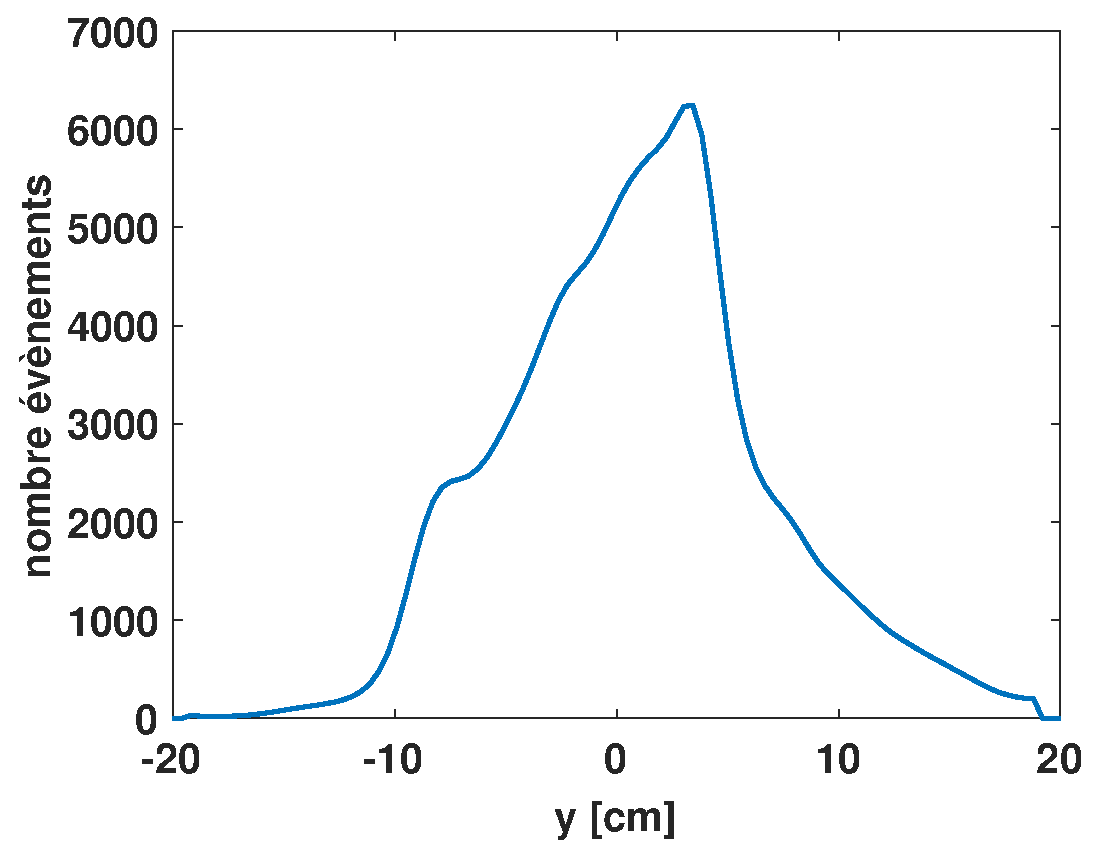
\includegraphics[width=0.33\textwidth]{./Figure/MLEM.eps}}\\
 \subfloat[\label{fig:fig_Estimation_Camera_CC_NURBS_Poisson_LC}]{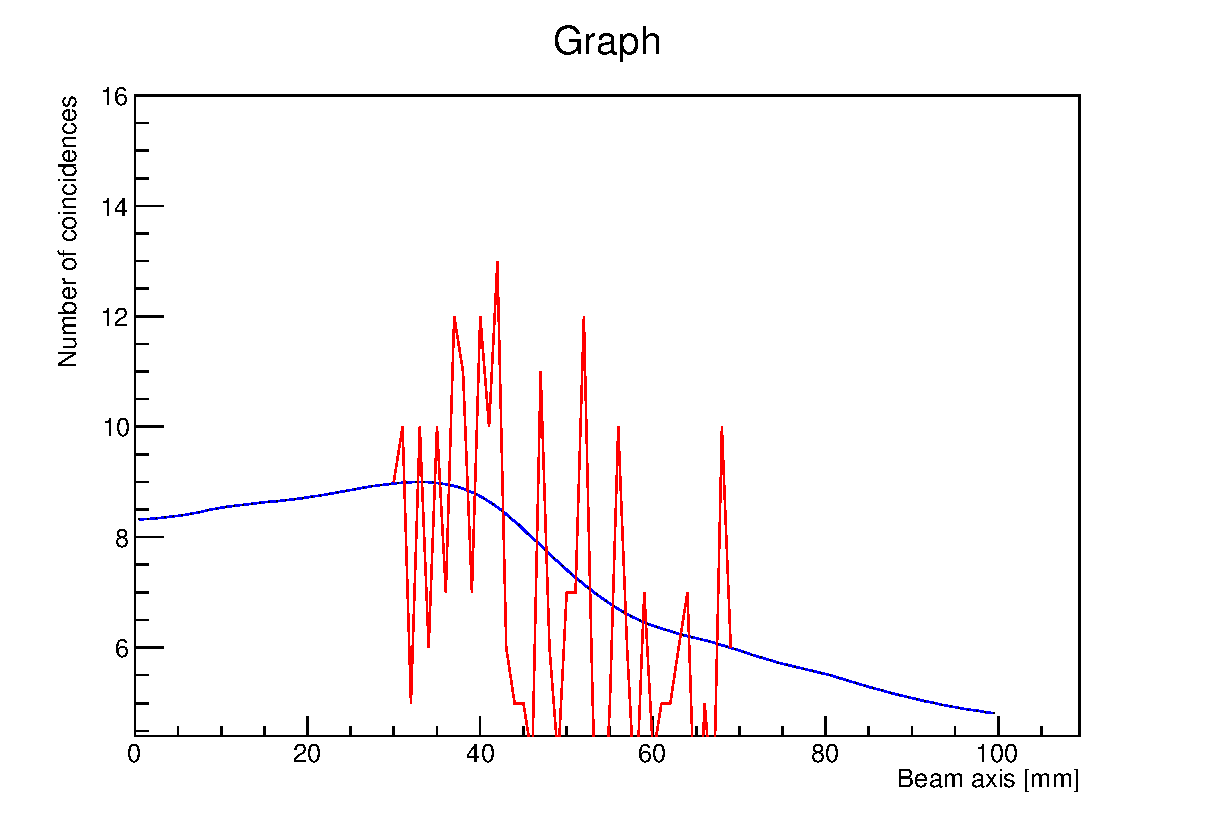
\includegraphics[width=0.33\textwidth]{./Figure/2017-08-02_Poisson_Nurbs_1e8_Article_LC.eps}}
 \subfloat[\label{fig:fig_Estimation_Camera_CC_NURBS_Poisson_MLEM}]{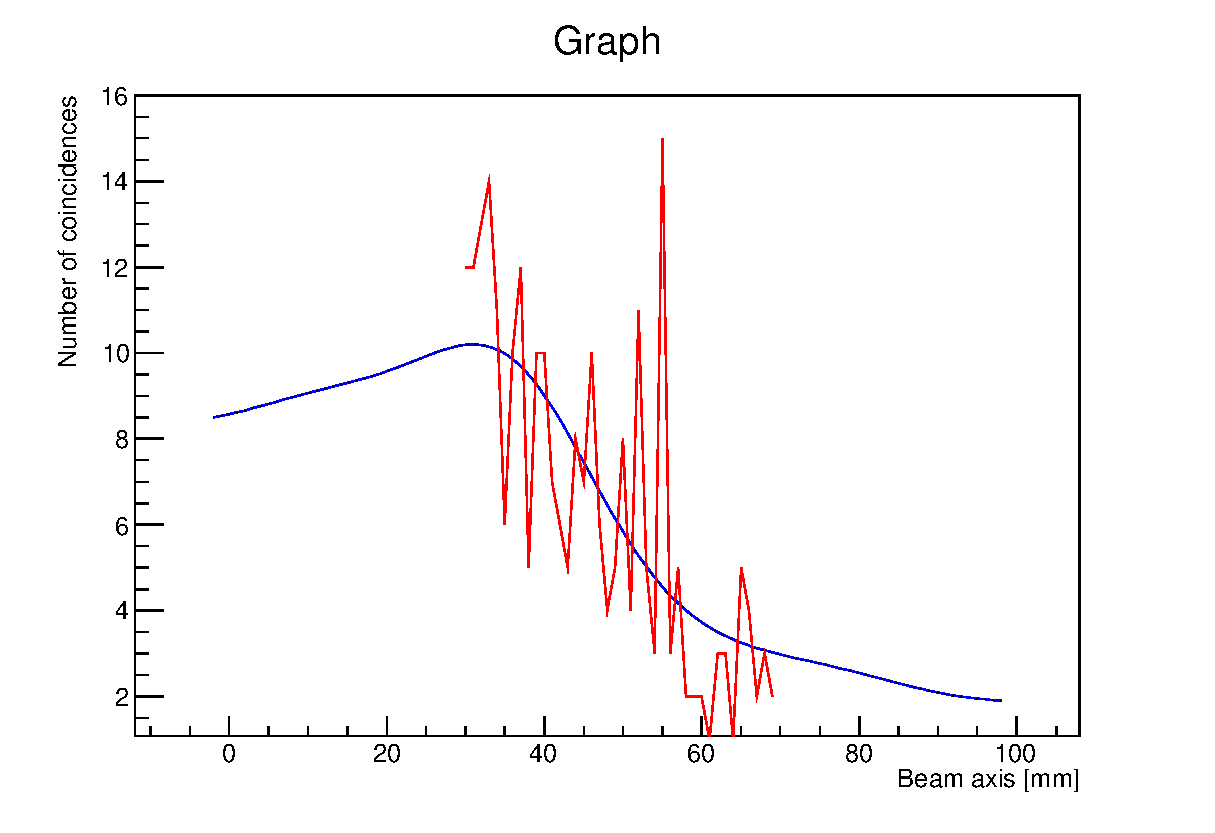
\includegraphics[width=0.33\textwidth]{./Figure/2017-08-02_Nurbs_Poisson_1e8_Article_MLEM.eps}}\\
  \subfloat[\label{fig:fig_Results_Chi2_Distribution_Variation_CC_simulation_Hadronth_LC}]{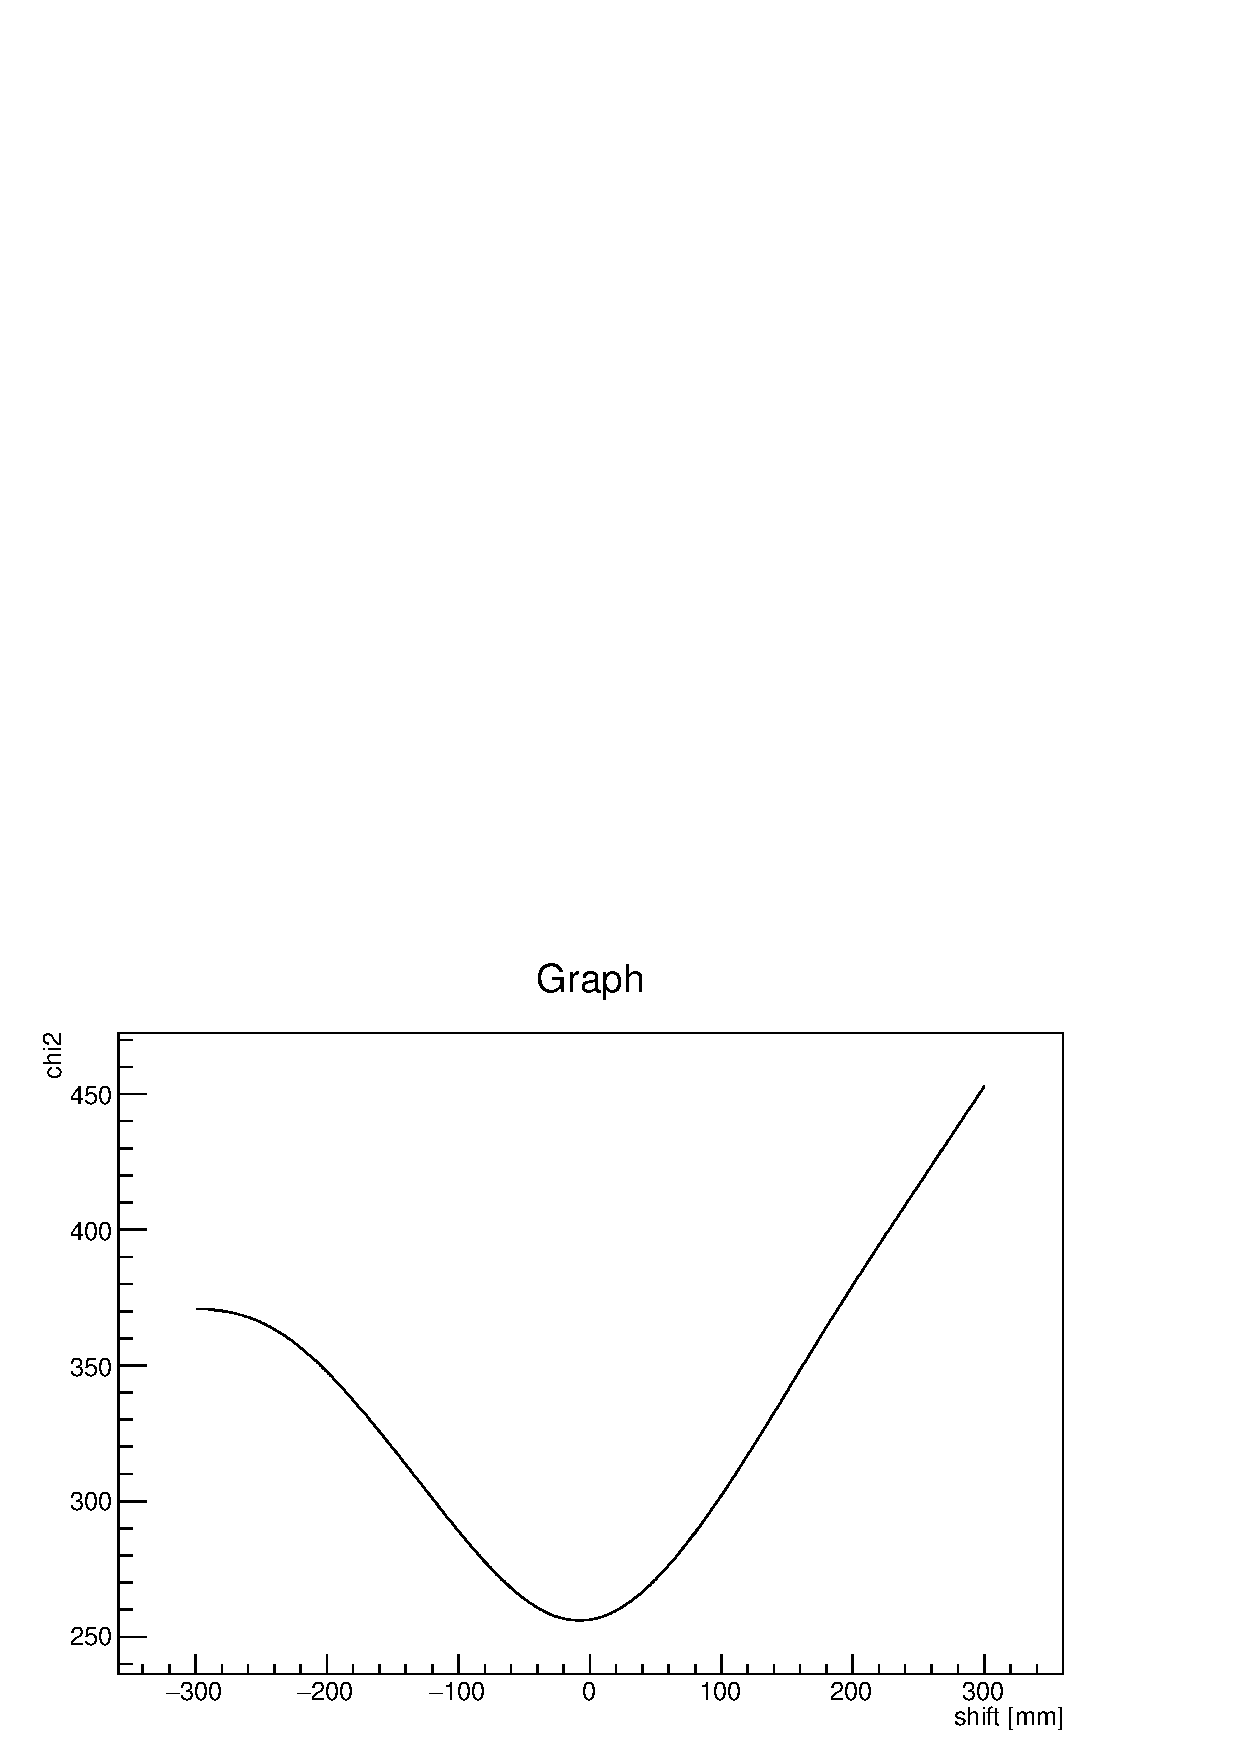
\includegraphics[width=0.33\textwidth]{./Figure/2017-08-02_Distribution_Chi2_1e8_LC.pdf}}
 \subfloat[\label{fig:fig_Results_Chi2_Distribution_Variation_CC_simulation_Hadronth_MLEM}]{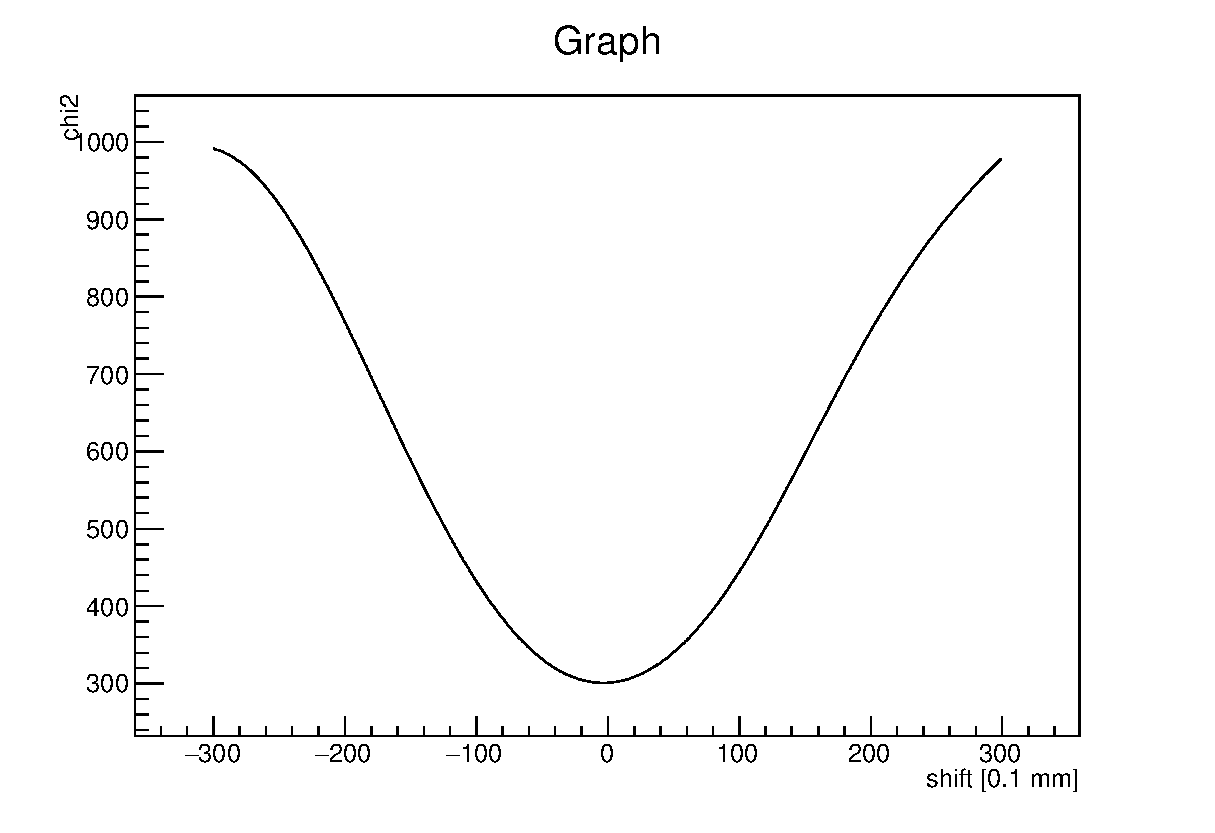
\includegraphics[width=0.33\textwidth]{./Figure/2017-08-02_Distribution_Chi2_Results_binning_1mm_ShiftNurbs0_1mm_1e8_article_MLEM.eps}}\\
  \subfloat[\label{fig:fig_Results_Precision_Distribution_Variation_CC_simulation_Hadronth_LC} ]{\includegraphics[width=0.33\textwidth]{./Figure/2017-08-02_Distribution_finale_1e8_Article_LC.pdf}}
 \subfloat[\label{fig:fig_Results_Precision_Distribution_Variation_CC_simulation_Hadronth_MLEM} ]{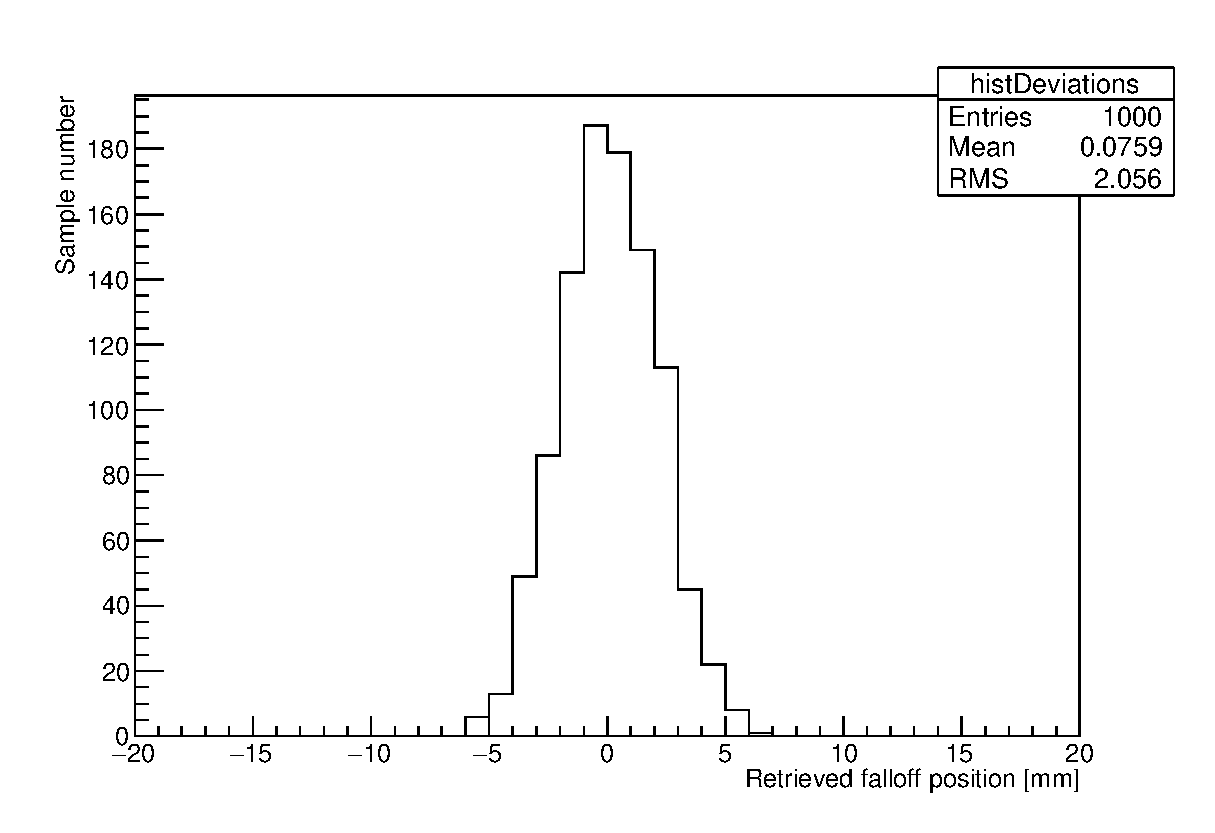
\includegraphics[width=0.33\textwidth]{./Figure/2017-08-02_FallOff_Results_binning_1mm_ShiftNurbs0_1mm_1e8_Article_MLEM.eps}}
  \label{}
\end{figure}

% b) 2016_10_20_Volume_100x200x5_voxels_and_size_20x40x1_Protons_1e10_1coinc_NoCutSum_sans_MatriceSensibility_bordYplusmoins-3_bordXplusmoins-3_cutx_Filtre_median_iteration_Profil_Y_CUTX_4cm_iteration_20.eps

